%\section{Experiment}\label{exp}


%講解實驗規劃與如何呈現數據
\section{實驗目的}
	
	為了改善室內定位的覆蓋率以及定位的精準度,我們利用建置虛擬相片的方法來增加照片的範圍及廣度。有了更多的取樣範圍,藉
由實驗來跟以前傳統的 SIFT 方法做比較。我們分成兩個實驗環境來說明方法所改善的定位數據:(1)可以控制的實驗環境、(2)一般
室內定位的環境。

	首先製造一個可以控制特徵點數量的環境,在這個環境中我們驗證每個固定距離內根據 SIFT 所涵蓋的特徵點數量作比較,增加
與物體的固定距離算出每個距離中的平均定位誤差,再算出定位誤差範圍的覆蓋率與傳統的照片影像定位作比較。在可以控制的定位環
境下我們根據這些實驗方法說明改善的成果,再把方法放建築一般實際的室內環境中作比較,最後呈現出改善的平均定位誤差與增加環
境所能定位的覆蓋率。為了完成這些實驗,所用到的設備為  Intel Core I5 2.0GHz 的CPU與 8 GB 的RAM,顯卡為了能夠使
用 CUDA 平行運算加速,所採用的是 Nvidia 的顯示晶片。

%1. Controlled Enviornment 
\section{可控制環境定位數據比較}


% 控制環境實驗目的與成效描述
\subsection{可控制環境實驗方法}
	建立可以控制的實驗環境主要目的為在可以控制的特徵點環境下與一般平面影像定位做比較,藉由實驗驗證出有更好的定位覆蓋率
與更小的平均定位誤差。在根據有限景物數量的環境下,將待定位的照片依距離增加,生成出格狀的位置的照片定位點,每個定位點前後
都有固定的間距距離,利用這些待定位照片,分別用三種方法比較實驗結果。

	一開始建置實驗環境,我們將這些定位照片分布在 4公尺 X 5公尺的環境大小內,而景物的分布在 1.5公尺 X 0.7公尺的大小範圍內, 
Kinect 攝影機放置在距離景物 0.5公尺前的地方,利用 Kinect 攝影機拍照取得深度照片與待定位的照片。如\ref{table:Controlled 
EV parameters}所示,在兩個控制環境的實驗中,利用不同的定位環境、不同的間距以及不同待定位圖片的數量來做實驗比較。
		
\begin{table}[htbp]
  \centering
  \caption{控制環境實驗參數設定}
    \begin{tabular}{rrr}
    \toprule
    實驗設定 :  & 控制環境 1 & 控制環境 2 \\
    \midrule
    待定位照片數量 : & 45 張  & 54 張 \\
    間距寬度 : & 0.5m & 0.5m \\
    間距長度 : & 0.75m & 0.5m \\
    \bottomrule
    \end{tabular}%
  \label{table:Controlled EV parameters}%
\end{table}%


\subsection{可控制環境實驗數據分析}

	為了證明在可以控制的環境下有比較好的定位結果,將實驗分成三個部分做討論:
	
\begin{itemize}
  \item (1) 特徵點數量分布分析
  \item (2) 定位誤差分布分析
  \item (3) 定位精準度覆蓋率以及平均定位誤差
\end{itemize}
		
\subsubsection{特徵點數量分布分析}

	這個實驗目的是要看出根據景物的距離增加與特徵點數量的關係圖,實驗的作法是先在待定位圖片的第一排中間設為圓心,如
\ref{fig:CoverDisk}所示。根據這個圓心將圓的半徑以 0.5公尺的長度增加,依據每個圓之間所能覆蓋的特徵點位置做特徵點數量的總和並算
出平均值,藉由圖中的趨勢看出特徵點數量的變化。

\begin{figure}
\begin{center}
  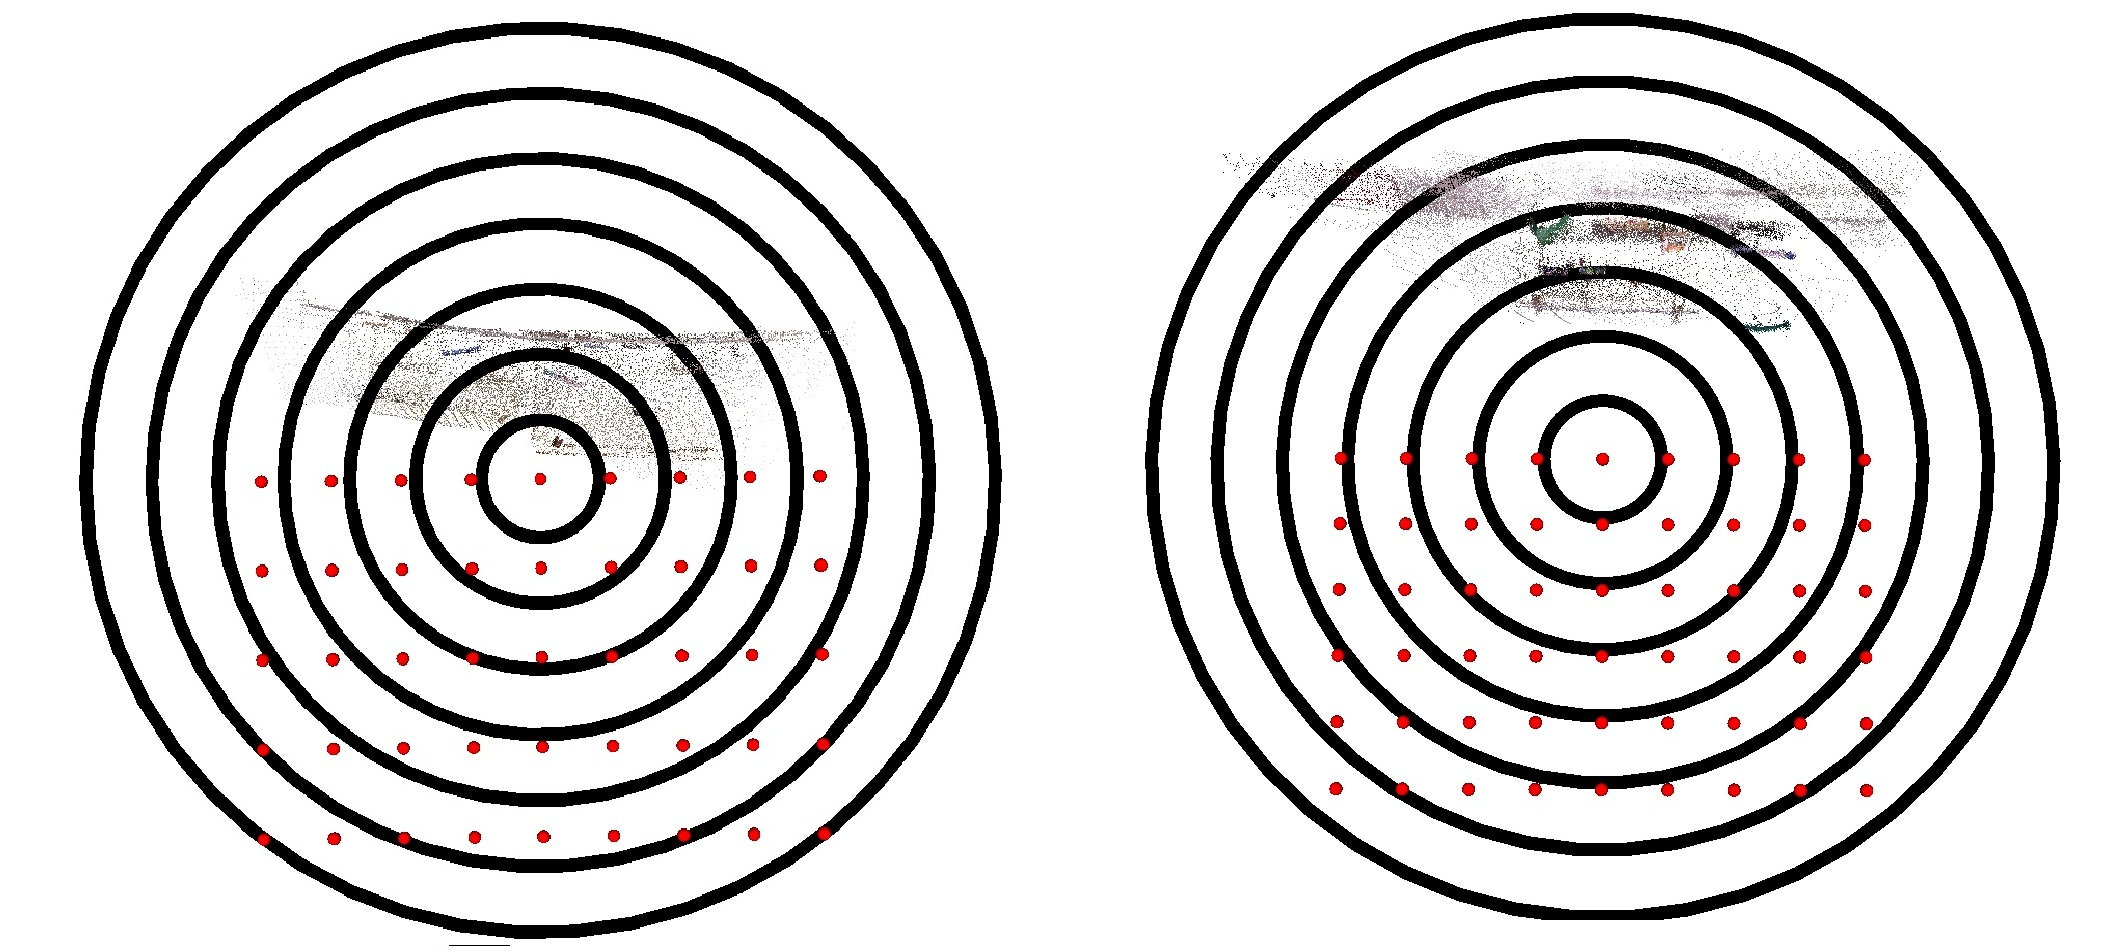
\includegraphics[width=1.0\textwidth]{figures/CoverDisk.jpg}
  \caption{依照同心圓的覆蓋算出每個半徑內的每張圖的特徵點平均數,左.控制環境 1 右.控制環境 2}
  \label{fig:CoverDisk}
\end{center}
\end{figure}
	
	如圖所示,橫軸表示與景物之間的距離增加,縱軸為特徵點的數量,三條線分別代表 1.2D隨機排列的攝影機影像位置,2.3D隨機排列的虛擬
攝影機影像位置與 3.3D格狀排列的虛擬攝影機影像位置,一開始距離越近根據2D影像所找出的影像特徵點也越多,符合實際的情況,但之後的趨
勢分布呈現卻發現距離越遠平面影像所找出的特徵點減少許多,表示說2D平面影像因為受到攝影機位置取樣的關係都侷限在景物附近,導致距離越遠
卻沒有好的匹配影像做比對,但是3D虛擬影像的好處在於可以分布在整個環境區域中模擬平面影像所照出的照片,所以特徵點的數量不會因距離增加
而有太大的改變,對於之後的定位精準度也不會因為距離增加而導致定位誤差有明顯擴大的影響。
			
	
\begin{figure}
\begin{center}
	
	
\end{center}
\end{figure}
	
	
	

%2. Indoor Localization
